\documentclass[11pt]{book}
\usepackage{amsmath}
\usepackage{graphicx}
\usepackage{mathtools}
\usepackage[]{verbatim}
\usepackage[]{qtree}
%Gummi|065|=)
\title{\textbf{Numerical Computation}}
\author{Ege Emir Ozkan}
\date{}

\begin{document}
\maketitle
\chapter{Sorting}

\section{Selection Sort}

\[
\]

Take this from Oguzhan

\section{Merge Sort}

\subsection{Merging Two Sorted Arrays}
Take this from Oguzhan

\subsection{Sorting using Mergesort}

\begin{figure}
\caption{Mergesort Algorithm in C}
\verbatiminput{algorithms/02-merge_sort.cverbatim}
\end{figure}
\chapter{Asymptotic Analaysis}

\paragraph{Instead of saying $f(n) \in \Theta(g(n))$, we say $f(n) = \Theta(g(n))$}
\section{Asymptotic Notation}

\paragraph{Functions defined on $IN = \{0, 1, 2, 3, ...\}, f(n) = an^2 + bn + c \rightarrow \Theta(n^2) as n \rightarrow \infty$ given $ g(n), \Theta(g(n))$ is the set $\Theta(g(n)) = \{f(n): \exists c_1, c_2, n_0 > 0$ such that $0 \leq c_1 g(u) \leq f(n) \leq c_2 g(n) \forall n \geq n_0\}$}

\begin{figure}[h!]
	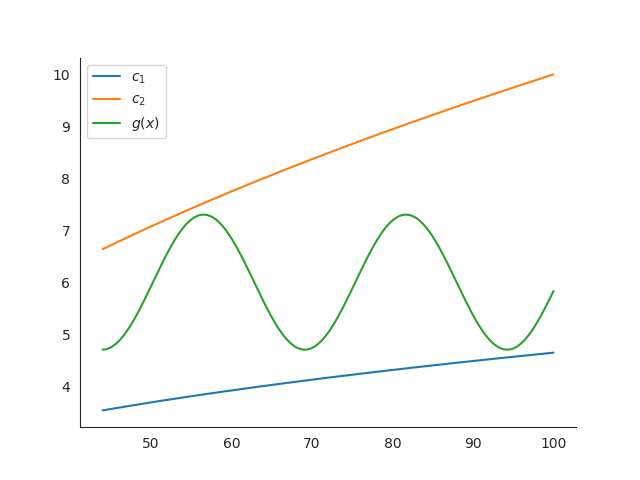
\includegraphics[scale=0.7]{figures/02_complexity.png}
	\caption{Complexity of functions}
\end{figure}

\[ \frac{1}{2}n^2 - 3n = \Theta(n^2)\]
\[ c_1n^2 \leq \frac{1}{2} - \frac{3}{n} \leq c_2\]
\[c_1 \leq \frac{n - 6}{2n} \leq c_2\]

For example, $6n^3 \neq \Theta(n^2)$ basically, all this boils down to:

\begin{equation}
p(n) = \sum_{i = 0}^d a_i n^i = \Theta(n^d)
\end{equation}

\section{O notation (big-Oh)}

\begin{equation}
f(n) = \Theta(g(n)) \Rightarrow f(n) = O(g(n)), \Theta(g(n)) \subseteq O(g(n))
\end{equation}


$g(n)$ is an asymptotic upper bound for $f(n)$, If an algorithm such as insertion sort has different best and worst cases, such as for insertion sort $\Theta(n)$ best case and $\Theta(n^2)$ for worst case, we say it has an $O(n)$, such that for an algorithm f, if $f = \Theta(k(x))$ for worst case and $f = \Theta(g(x))$ for best case, we say that $f = O(k(x))$

\subsection{Growth of an algorithm}

\subsection{Analysis of Recursive Algorithms}

Reccurance equation describes the runtime of rectursive algorithm in terms of smaller algorithms.

\[
T(n) = 
\begin{cases}
	\Theta(1) & n \leq C \\
	aT\left(\frac{n}{b} \right) + D(u) + C(u) & \text{otherwise} \\
\end{cases}
\]
Where $D$ is divide time and $C$ is combine time.

\subsubsection{Analaysis of Mergesort}
\begin{equation}
T(n) = 
\begin{cases}
	\label{eqn:merge}
	\Theta(1) & n \leq 1 \\
	2T\left(\frac{n}{2} \right) + \Theta(1) + \Theta(n) & n > 1 \\
\end{cases}
\end{equation}

And therefore, the computational complexity of merge sort is

\begin{equation}
T(n) = 2T\left( \frac{n}{2}\right) + \Theta(n)
\end{equation}

\subsubsection{The Recursion Tree Method}

\Tree [ .$Cn$ [ .$C\frac{n}{2}$  $C\frac{n}{4}$ $C\frac{n}{4}$ ] [ .$C\frac{n}{2}$ $C\frac{n}{4}$ $C\frac{n}{4}$ ] ]

\break
From here, it is easy to see each level has a total complexity of $Cn$, and the recursion tree is of depth $\log_2(n)$ therefore the whole program has a total complexity of $\Theta(n \log_2(n))$, this can also be proven from a method where one would solve the recursion equation \ref{eqn:merge}.

\subsubsection{Basic Reccurances}

For a loop eliminating a single item, calculations end up to $\Theta(n^2)$, as  for a recursive program that halves the input in constant time.
\end{document}

